
\section{Case studies}\label{sec:algorithm}
 {\color{red} fix this section - anyone?}

First
 While the SE-dynamical core, has demonstrated scaling to approximately 300K hardware cores \cite{came} on a ultra high $1/8^\circ$ degree resolution, simulating climate at such high resolutions is still fundamentally not feasible due to the extreme cost of these simulations a very large core counts.  Even $1/4^\circ$ degree resolution are effectively limited to approximately 10-20K cores due to simulation costs and scalability limitations.  


[Why we focus on homme]


The High-Order Method Modeling Environment (HOMME) atmospheric dynamical is used by the Community Atmosphere Model (CAM) as the default dynamical core for very high $1/4^\circ$ resolution simulations.   The HOMME dynamical core which can consume 30-88\% of the total cost of the CAM has a key impact on the overall scalability of CAM and CESM.HOMME uses a cubed-sphere topology where each face of the cube is projected onto a sphere to generate a global computational grid.  HOMME uses a spectral element method to discretize in the horizontal and a finite difference approximation \cite{simmons:1981} in the vertical. A continuous Galerkin finite-element method \cite{taylor:1997} is used for the spectral element method. The integrals used in the Galerkin formulation are computed from a Gauss-Lobatto quadrature rule within each element.  HOMME decomposes each time-step into components and the equation, for a compressible fluid with hydrostatic and a shallow water approximations, can be written in terms of a vector U containing the prognostic state variables (velocity, temperature, and surface pressure) as: 
dU/dt = F + D + A + T + R
Where F represents the forcing from physics, D the dissipation, A the dynamics from the primitive equations, T the tracer advection, and R the vertical remapping of the mass and momentum variables. A diagram of the overall computational flow of the HOMME algorithm is provided in Figure \ref{fig:homme-alg}. 

HOMME solves these equations in a time-split fully-explicit form. For time-steps involving the forcing (F) and dissipation (D) terms, a forward Euler time- scheme is used. The dynamics (A) and tracer advection (T) are computed using an N-stage Runge-Kutta time-scheme. The dynamics (A) computes the primitive equations prognostic variables. The tracer advection (T), is based on a finite-volume algorithm and advances the specific humidity, liquid water, ice variables, and additional tracer constituents. For advection, a vertical Lagrangian approach used \cite{lin:2004} where the horizontal advection on Lagrangian vertical levels is followed by remapping (R) the mass and momentum variables back to the reference vertical levels at the end of the time-step.

\begin{figure}[tbp]
 \begin{center}
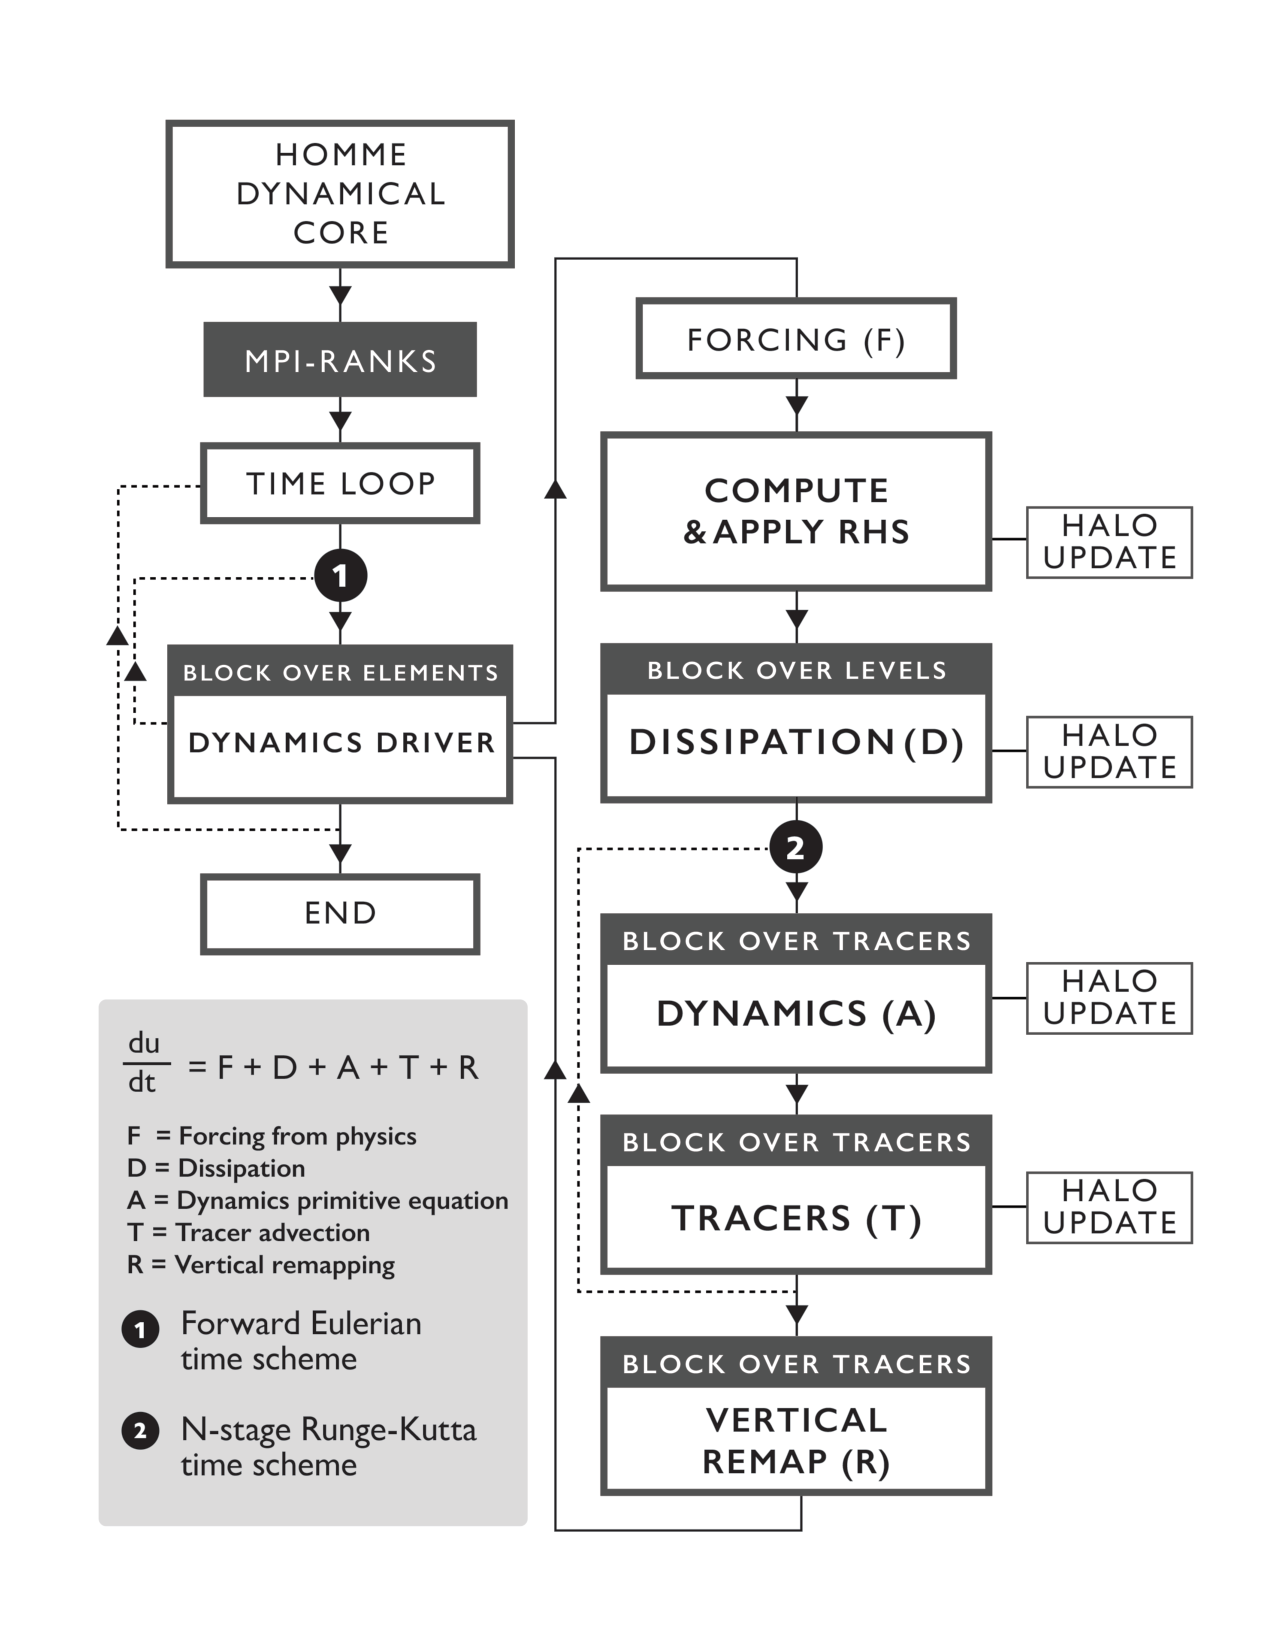
\includegraphics[width=12.0cm]{figures/HOMME-v01.pdf}
\end{center}
\caption{The computational phases within HOMME.}
\label{fig:homme-alg}
\end{figure}
